\section* {1.3  Метод простых итераций. Метод Зейделя}

\subsection{Постановка задачи}
Реализовать метод простых итераций и метод Зейделя в виде программ, задавая в качестве входных данных матрицу системы, вектор правых частей и точность вычислений. Используя разработанное программное обеспечение, решить СЛАУ. Проанализировать количество итераций, необходимое для достижения заданной точности. 

{\bfseries Вариант:} 22

\begin{cases}

& -18x_1+9x_2-1x_3-8x_4 = -60 \\
& 6x_1+22x_2+9x_3 = -109 \\
& -4x_1+2x_2-16x_3+9x_4 = -103 \\
& 1x_1+6x_2-1x_3-14x_4 = -33 \\
\end{cases}
% \pagebreak

\subsection{Результаты работы}
\begin{figure}[h!]
\centering
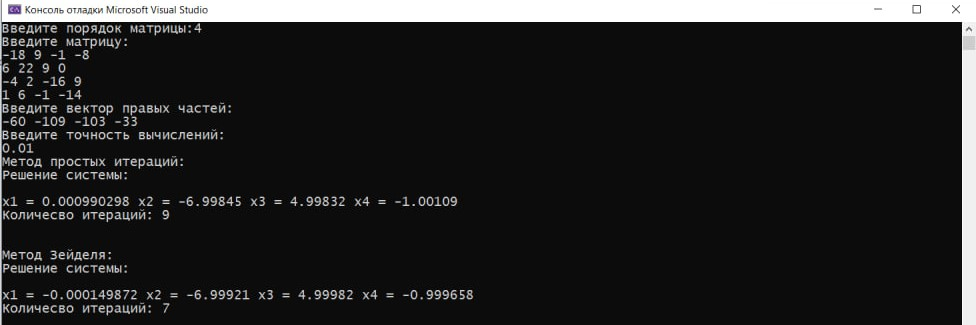
\includegraphics[width=.9\textwidth]{lab1.3}
\caption{Вывод программы в консоли}
\end{figure}

% \vfill

% \begin{figure}[h!]
% \centering
% 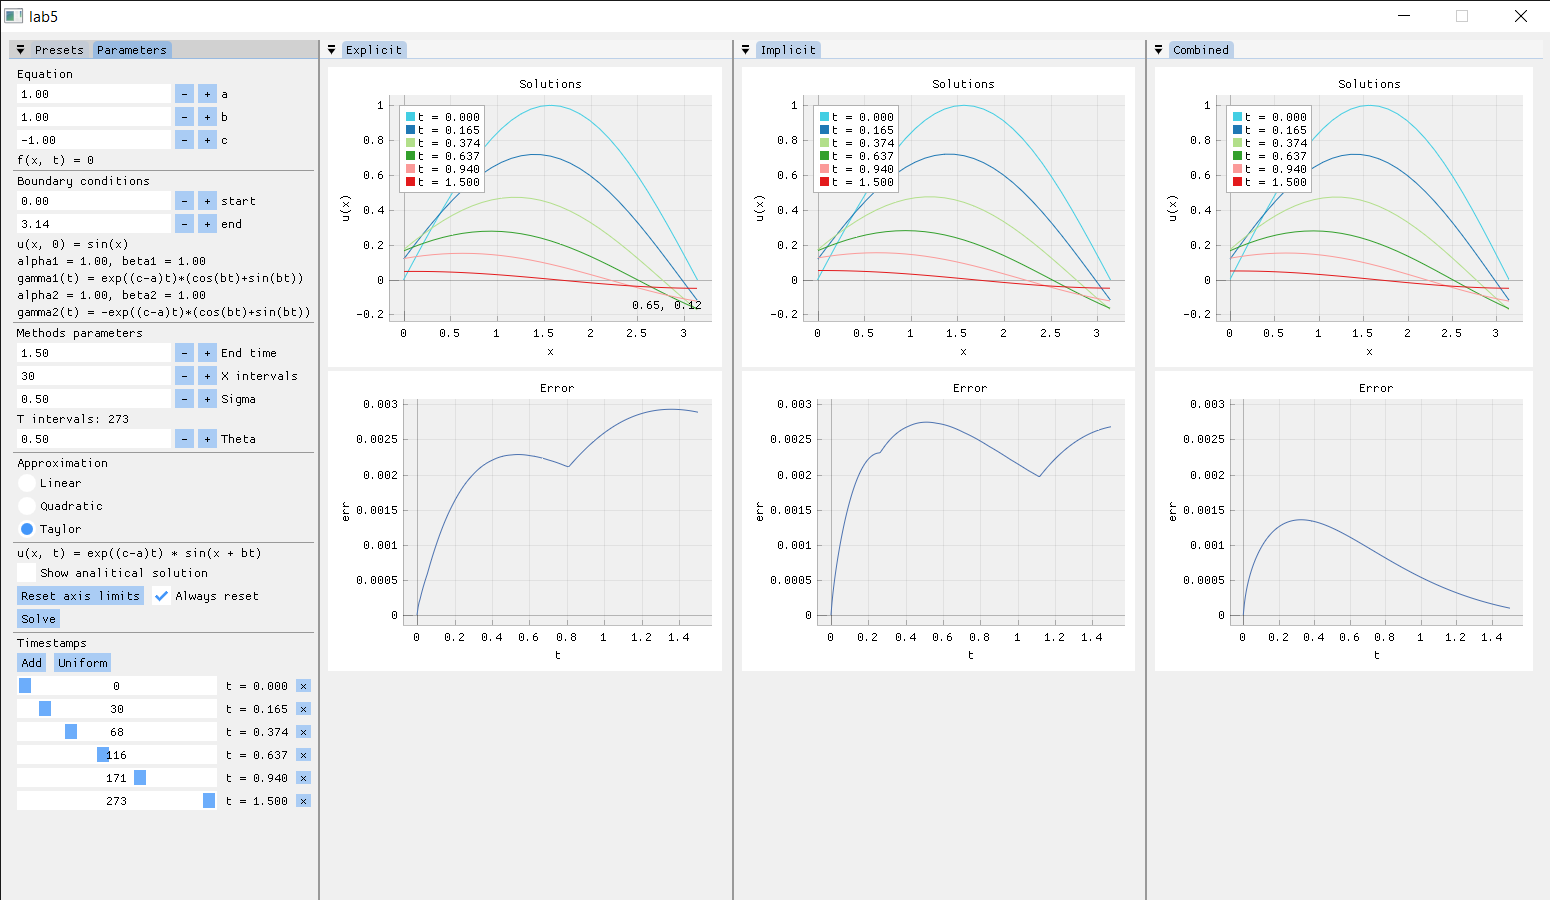
\includegraphics[width=.9\textwidth]{lab5_taylor}
% \caption{Решение с аппроксимацией граничных условий со вторым порядком}
% \end{figure}
\pagebreak

\subsection{Исходный код}
% \lstinputlisting[language=C++]{matrix.cpp}
% \begin{lstlisting}
\lstinputlisting{include/lab1_3.cpp}
\lstinputlisting{include/matrix.cpp}
\lstinputlisting{include/matrix.h}
% \end{lstlisting}
% \lstinputlisting{matrix.cpp}
% {../../include/matrix.cpp}
% \pagebreak
% \lstinputlisting[title=\texttt{parabolic\_pde.hpp}]{../../include/partial_differential/parabolic_pde.hpp}
% \pagebreak
% 